\section{\tool}
\label{sec:badusb}
\subsection{Threat Model}

We build our threat model on the basic assumptions that common users without
technical background would not treat normal-looking \ac{USB} device as malicious and be cautious about them. This assumption is consistent with existing works~\cite{JFCImpact}. Moreover, we neglect the
effect of notifications from \ac{USB} devices, as users may not have the knowledge to fully understand such notifications. In
fact, during our experiment, no device had security notifications raised about
suspicious \ac{USB} devices and only mobile devices had raised a charging notification
about our \tool, which may not be a sufficient warning for users.

We also assume the victim's device is equipped with fully functional \ac{USB} 3.x
protocol and \ac{USB} Type-C connector. As the \ac{USB} 3.x standard is
common nowadays, this assumption can be fulfilled in recent
devices.

%\subsection{Motivation}
%\noindent\outline{Limitation of Rubber Ducky}\\
%\outline{Our functionality different mode listing?}\\
%\hongyi{The following mode is to be further decided}
%\outline{Automatic Scripting Mode}\\
%\outline{Remote Control Mode}\\
%\outline{OCR/QR Recognition Mode}\\

\subsection{Implementation}
%\noindent\hongyi{The following mode is to be further decided}\\
%\outline{DETAIL of each mode}\\ \outline{Automatic Scripting Mode}\\
%\outline{Remote Control Mode}\\ \outline{OCR/QR Recognition Mode}\\

As introduced in Section~\ref{sec:related_work},
existing works~\cite{rubber,badusb,
rubberducky2020,usbbypassing,iseeyou,usbdriver} focus on BadUSB attacks.
Many of these take advantage of the \textit{trust-by-default} policy of PC,
pretend to be normal \ac{HID} devices and utilize \ac{USB} protocol to perform attacks.
However, these attacks suffer from various drawbacks: \ding{182} attackers can
only simulate limited types of devices such as \acp{HID} (like keyboards and mice)
and disks, which makes the attacks less effective; \ding{183} accurate attacks
could not be performed due to lack of \ac{UI} status. Whatever \ac{HID} the
attackers simulate their \ac{USB} devices to be, they could not obtain the \ac{UI} to
check the status information, which makes it nearly impossible to carry out
their attacks precisely or know the effects after attacks.

%Though BadUSB devices\cite{badusb} like Rubber Ducky\cite{rubber,
%rubberducky2020} emulates as a HID device enabling various arbitrary execution
%attacks, fetching feedback from the victim is much more limited.
Based on the drawbacks introduced above, several defense mechanisms were
proposed. For example, GoodUSB~\cite{tian2015defending}
implemented a authorization procedure when a new device is plugged in and blocks other functions excepted authorized ones.

In this work, we utilize the new features of \ac{USB} 3.x~\cite{usb31,usb32} to
address the problem above.  Benefiting from the latest protocol, we simulate
external display and thus obtain the video stream to perform accurate
attacks. However, we still unable to bypass defenses like GoodUSB~\cite{tian2015defending}, which completely blocks unauthorized functionality. This will be further discussed in Section~\ref{sec:discussion}

As there were various BadUSB implementations available, this work focuses on our new extensions. Next, we first introduce the
components we used in \tool, then we focus on the three different attack modes
we implement for various scenarios.

\subsubsection{Attack Model}

Figure~\ref{fig:attack_model} shows the architecture of our attack model. \circled[text=white,fill=myyellow]{\footnotesize{1}} represents the victim's devices; \circled[text=white,fill=myyellow]{\footnotesize{2}} is our \tool; \circled[text=white,fill=myyellow]{\footnotesize{3}} is the attacker's remote PC. The details of each component in \tool are as follows.

%\fengwei{We need to
%explain the figure. What are the boxes? Where is victim? Where is the attacker?
%The list below only shows the internal components in the malicious \ac{USB} device.
%We might also consider to explain this in the Figure caption.}

\begin{itemize}
	
	\item\underline{USB 3.x Hub} exports the \ac{USB} 3.x connector into various ports, like DisplayPort, \ac{USB} 2.0 port, etc.
	
	\item\underline{Video Capture Card} converts DisplayPort signal into compatible data, which is later processed by the Single Board Computer (i.e., an embedded computer).
	
	\item\underline{\ac{HID} Emulator} emulates \ac{HID} device which can be controlled from the attacker.
	
	\item\underline{Single Board Computer} processes video stream from the victim via the Video Capture Card or sends commands to the victim via \ac{HID} Emulator.
	
	\item\underline{Wi-Fi/GSM Module} transmits the sensitive data or receives commands to/from the remote attacker PC.

\end{itemize}


\begin{figure}[t]
	\centering
	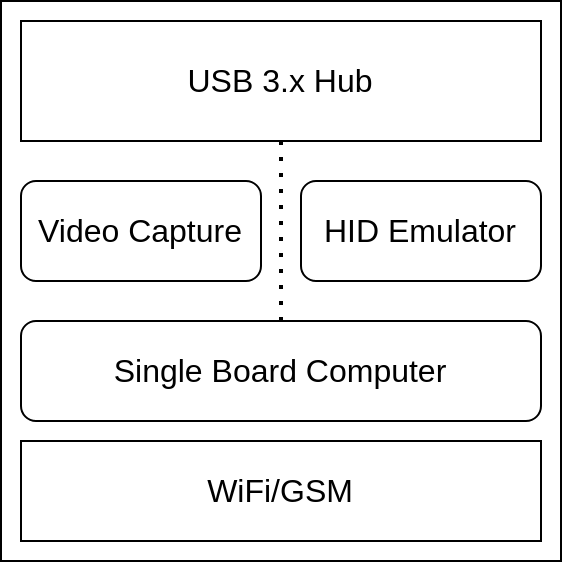
\includegraphics[width=\linewidth]{./Figs/attack_model.png}

	\begin{tabular}{ll}
	\circled[text=white,fill=myyellow]{\footnotesize{1}} Victim's Devices    &\circled[text=white,fill=myyellow]{\footnotesize{2}}~\tool\\
	\circled[text=white,fill=myyellow]{\footnotesize{3}} Attacker's Remote PC
	\end{tabular}

	\caption{Attack Model.}%\shuqing{Need to be more compact.}
	\label{fig:attack_model}
\end{figure}

\textbf{\ac{HID} Emulation Mode.} This mode majorly relies on the ``\ac{HID} Emulator'' in the Figure~\ref{fig:attack_model} to
send constructed \ac{HID} packet to the victim. These constructed \ac{HID} packets are
interpreted by the victim as valid keystrokes and mouse moves. Thus, the
attacker can executes arbitrary scripts on the victim's device. This is the
function of the original BadUSB. Based on this, we made the following
improvements.

First, as \tool has established a feedback channel using \ac{USB} 3.2 protocol, when performing keystroke and mouse movement injection, attacker can obtain real-time feedback from the victim's devices. This feedback allows an attacker to tell whether the previous attack succeeded and decide what to perform next. Existence of such feedback channel largely strengthen the attack ability of \tool.

Moreover, as the mouse relies on the visual feedback to work properly, its
emulation and automation were not supported by the original version of BadUSB.
Yet with the video output support from \ac{USB} 3.x, our \tool implements a
full-functional mouse emulation. This function enables attacks toward pure \ac{GUI}
programs and shows attacks in the mobile attack scenarios. Details can
be obtained in Section~\ref{sec:experiment}.

The advantage of this mode is that it archives defense bypass and attack
feedback with video streaming.  
%\fengwei{I don't understand the sentence below.}\hongyi{Fixed, I think it's redundant and less important}
%As mentioned above, we only require video stream at the beginning (defense
%bypass) and the end (result feedback) of the attack.
Also, with mouse
supported, \tool extends the original BadUSB attack and results in further attacks in
mobile devices.

\textbf{Video Capture Mode.} \tool under this mode does not emulate other
USB device and solely relies on the video stream function of \ac{USB} 3.x; it uses
``Video Capture'' component as shown in the Figure~\ref{fig:attack_model} to transmit the stream to the embedded ``Single Board Computer''.
%\fengwei{What is embedded computer? Do we define this in the previous\hongyi{Fixed by using the term mentioned in Figure}
%text?}. 
The victim's device would mistakenly treat \tool as an external monitor
and output its video stream. This stream is latter processed by the embedded
computer to extract sensitive data.

When running in this mode, \tool passively processes the victim's video stream
and detect for ``valuable'' private data.  The data is considered as
``valuable'' or not is decided by a customized detector, we implemented a simple
payment code detector for the poof-of-concept purpose, which demonstrates that we successfully transfer money from a victim to an
attacker. More detail can be obtained in Section~\ref{sec:experiment}.

It is worth mentioning that \tool under this mode is completely passive, making
it hard to be detected. With different detector implemented, \tool
under this mode is capable of serving more purposes.

\textbf{Full Control Mode.} In \tool, we have implemented all components
required to control a computer/mobile device completely, including a video stream
and a keyboard/mouse emulation. Thus with all components enabled, not only
the victim's device treat \tool as an external display, but also a valid \ac{HID}
input source. Hence we can archive complete hijack of victim's device.

\tool under this mode follows a simple logic. \tool receives video stream
from the victim's device and redirect it to the attacker via GSM/WiFi. In the
meanwhile, \tool also receives keystrokes and mouse movement from the attacker
through GSM/WiFi and replays them to the victim by the \ac{USB} emulation.

This mode enable attacker to perform delicate operations that are beyond
automation. Moreover, this mode provides a backdoor that does not require host
network and thus is undetectable by the firewall running on the host machine.
%\hongyi{I think this is a quite good selling point?}\shuqing{Agree with
%Hongyi.}

The advantage of this mode is that it can completely hijack the victim device
and provide a backdoor beyond detection of firewalls; however, this complete control
also comes with the price of high power consumption and risk of being detected
by the user.

